% INNAN DU COMMITAR!
% Uppdatera datum
% Uppdatera version
%-----
% Document name

\documentclass[10pt,a4paper]{article}
\usepackage[utf8]{inputenc}
\usepackage[english]{babel}
\usepackage{amsmath}
\usepackage{amsfonts}
\usepackage{amssymb}
\usepackage{graphicx}
\usepackage{geometry}
\usepackage{enumitem}
\newcommand{\tsss}{\thesubsubsection}

\title{PostCardBuddy}
\author{Team C}

\begin{document}
\begin{titlepage}
\newgeometry{left=2cm,top=1cm,right=2cm}
\newcommand{\HRule}{\rule{\linewidth}{0.5mm}}


\begin{flushright}
December 1, 2015 v1.11\\[3cm]
\end{flushright}


\centering
\textsc{\LARGE Team C}\\[0.5cm]

\HRule \\[0.4cm]
{ \huge \bfseries PostCardBuddy}\\[0.3cm]
{\Large \bfseries System Requirements}\\[0.4cm] % Title of your document
\HRule \\[1.5cm]

\vfill
\begin{flushleft}
\textit{Authors of this document:}\\
Emma Albertz\\
Caroline Brandberg\\
Linnéa Claesson\\
Billy Johansson\\
Johan Ju\\
Jacob Mejvik\\
Carl Rynegardh
\end{flushleft}

\end{titlepage}
\pagenumbering{gobble}



%\begin{center}
%\textit{\large Version History}
%
%    \begin{tabular}{ | l | l | l | p{5cm} |}
%    \hline
%    \textbf{Version} & \textbf{Date} & \textbf{Responsible} & \textbf{Description} \\ \hline
%    1.0 & 2015-10-14 & EA, LC & Baseline\\ \hline
%    \end{tabular}
%\end{center}



\setcounter{tocdepth}{2}
\tableofcontents
\newpage
\pagenumbering{arabic}

%-------------------------------------------------------------------%
%---------------------- Introduction -------------------------------%
%-------------------------------------------------------------------%
\section{Introduction}
This document is written within the context of the course Requirements Engineering at Lund Institute of Technology, which the authors are currently enrolled in. They have been provided with a project mission from another group, specifying a product they want to see developed. This group has also acted as the key customer. The intention of this document is to specify the requirements of this product, namely PostCardBuddy.


%-------------------------------------------------------------------%
%---------------------- Background ---------------------------------%
%-------------------------------------------------------------------%
% Extend background from PMv2
\section{Background}
Everybody likes receiving postcards, but the process of sending them is tedious and takes too much effort. This is what PostCardBuddy hopes to change. PostCardBuddy is a mobile application that will simplify the process, whether you want to be creative and design your own postcards or make it easy for yourself and use a template postcard based on your location and send it to everyone in your contact list. 

The application is perfect for every occasion you want to send a postcard. Grandma's birthday is coming up? Send a postcard of you and your cousins! Christmas is around the corner? Send everyone in your contact list a postcard of your cats! Away on vacation? Why not send a ready-made postcard that shows off the amazing beach to everyone in the office? Nobody needs to know it rained all week. 

PostCardBuddy is the perfect tool when you want to let someone know you are thinking of them, no matter the occasion.

%--------------------------------------------------------------------%
%----------------- System Requirements ------------------------------%
%--------------------------------------------------------------------%
% Different types of system requirements (e.g. data, function, quality) at different levels (e.g. goal, domain, product, design).
% Each requirement should have a unique identity (name or number) that is consistent between releases.
% A subset of the requirements should be prioritized.

% 3A) more than two types of requirement (e.g. data, function, quality), and more than three abstraction levels (e.g. goal, domain, product, design) 
% 4A) combine different degrees of completeness and different levels of abstraction
% 4C) provide explicit requirements rationale that reduce risks of misinterpretation.
% 4D) use hierarchies and requirements relations to manage evolving requirements structures.
% 5G) use prioritization to focus improvements of specification quality and elicitation efforts for a well motivated subset of requirements.

\section{Definitions and terms}
\begin{description}
\item[Device] Mobile device on which it is possible to download an use applications.
\item[Standard library] Library of pre-existing images in application.
\item[Phone gallery] User's existing image gallery on phone.
\item[Mobile user] Person who owns a smart phone. 
\item[Payment solution] A feature that makes it possible to charge the costumer in the application. 
\item[Payment service] A company who provides a payment solution for applications. 
\item[Personalized postcards] Postcards were the design is chosen by the person who sends the postcard. 
\item[Product]The application described in this Requirement Specification.
\item[Postal service] A company that delivers mail to private citizens.
\item[Recipient]The person which a postcard is addressed to.
\item[Printer of postcards] The company who delivers the postcards from the printer to the postal service. In this project the key customer.
\item[Supplier of images] The companies or persons who supply the application with images for the standard library.
\item[System] The application described in this Requirement Specification.
\end{description}

\section{System Requirements}

\subsection{Goal}
The product aims to establish the key customer in the postcard sending market and shall achieve this through the following goals:

\begin{itemize}
\item Simplify the process of sending postcards
\item Enable user to send personalized postcards
\item It shall be possible to generate revenue through the system
\end{itemize}

\subsection{Domain}
Write short text about contents of this section.

\subsubsection{Context Diagrams}
The context diagram of the product can be found in figure~\ref{fig:context}. This diagram shows the interface that the application PostCardBuddy will interact with and the stakeholders who will interact with the application.

There are two stakeholders that will interact directly with the application; the mobile user and the supplier of images. The mobile user is the one that will use the application for creating its personalized postcard. For the front of the postcard the user shall be able to select an image from the applications standard library. These images will be delivered from supplier, which are shown as \textit{Supplier of images} in the context diagram. 

The application needs various of functionality. Some of these functionalities will be used from the users mobile phone. The camera available from the users mobile phone will be used to enable the user to take a picture. The GPS location of the user shall also be provided from the phone. The GPS location will be used to select which pictures will be presented first from the standard library. The contacts available in the users phone will also be used to select recipients. These three permissions shall be confirmed by the user. The user shall also be able to send a digital postcard, via email. 

The user shall also be able to send a physical postcard. This will cost money, which will be taken care of by a payment service. When the payment is done there will be a franking of the postcard. Thereafter the postcard will be sent to a printer. The printer will be placed so that a supplier, shown as \textit{Printer of postcards} in figure~\ref{fig:context}, easily can pic up the card and deliver it to the postal service. The last stage in this chain is the stage where the postal service deliver the physical post card to the desired recipient. 

\begin{figure}[h!]
\centering
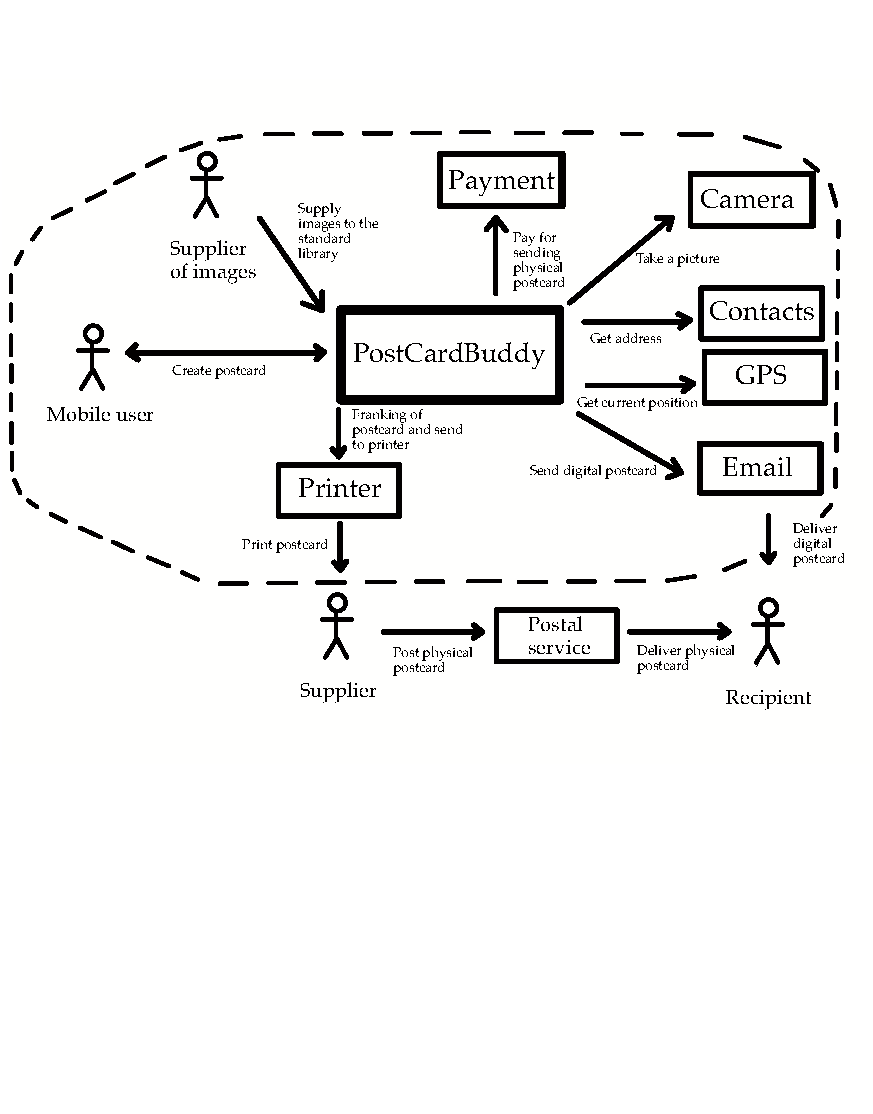
\includegraphics[width=0.7\textwidth]{ContextDiagram3.pdf}
\caption{Context diagram of product.}
\label{fig:context}
\end{figure}

\subsubsection{Stakeholders}
Some of the stakeholders for PostCardBuddy are presented in Table~\ref{table:stakeholder}. For each stakeholder there is a number to visualize how much prioritization each stakeholder have. The scale is from 1-5 where 1 represent a high priority and 5 a low priority.


\begin{table}[h!]
\centering
\label{table:deliv}
\begin{tabular}{|l|l|} \hline
\textbf{Stakeholder} & \textbf{Priority} \\
\hline
Mobile user & 1\\
\hline
Printer of images & 2\\
\hline
Postal service & 2\\
\hline
Payment service & 4\\
\hline
The existing application \textit{Riktiga Vykort} & 4\\
\hline
Developers & 3\\
\hline
\end{tabular}\\
\caption{Stakeholder prioritization}
\label{table:stakeholder}
\end{table}

\begin{description}
\item[Mobile user] was given the highest priority since they will be the ultimate users of the product and without them there will be no market.
\item[Printer of postcards] will act as the key customer, since they placed the order of the product, and thereby given a high priority. 
\item[Postal service] was given a high priority because they are considered a possible buyer of the application. 
\item[Payment service] was given a low priority. The payment service will be used only to provide the application with a pay-functionality, and therefore its low priority.
\item[The existing application \textit{Riktiga Vykort}]  is a competitor to the application. 
\item[Developers]  decide whether a functionality is reasonable or not.
\end{description}

\subsubsection{Tasks}
\begin {description}
\item[Work area:]  Vacation
\newline
Communicating with friends and family. Usually from a remote location with unreliable internet access. Typically sunny and overall poor working environment. Simplicity is key to capturing important moments. \newline
Users: Average smart phone user, used to little manual work. 

\item [Req 1.2.1.1] The system shall support tasks 1.1 and 1.2.
\item [Task 1.1] Send a postcard.
\begin {description}
\item \textbf{Purpose:} Take a picture. Edit the picture. Add a message. Add recipients. Send postcard.
\item \textbf{Precondition:} PostcardBuddy is running.

\item \textbf{Sub-tasks:}
\begin{enumerate}
\item Use the camera in the device to take a picture.
\item Allow basic editing of pictures.
\item Save pictures.
\item Add recipients from address book. 
\item Save finished postcard.
\item Preview postcard.
\item Send postcard to printer.
\end{enumerate}

\item \textbf{Variants:}
\begin{itemize}[label={}]
\item[1a] The user selects a picture from the personal gallery.
\item[1b] The user selects a picture from PostCardBuddy's standard library. 
\item[2a] Include editing of library pictures.
\item[4a] Manually add address.
\end{itemize}
\end{description}
\item [Task 1.2] History

\begin {description}
\item \textbf{Purpose:} View sent cards. View recipients. View cost.
\item \textbf{Precondition:} PostcardBuddy is running. 

\item \textbf{Sub-tasks:}
\begin{enumerate}
\item List sent postcards. 
\item Search sent postcards.
\item Summary of cost.  

\end{enumerate}
\item \textbf{Variants:}
\begin{itemize}[label={}]

\item[1a] No postcards sent. 
\item[2a] No postcards found for given search criteria. 

\end{itemize}
\end{description}
\end{description}



\subsubsection{Interfaces}
\begin {description}
\item [Req 1.2.2.1 Printer] The interface connecting PostCardBuddy and the printed postcards is an off-the-shelf printer.
\item [Req 1.2.2.2 Print files] The system sends image files to a printer. 
\end{description}

\subsection{Product}
Short text describing this section.

\begin{description}
\item [Req 1.3.1.1 Success notification] The user shall be notified when an order is sent from a device.
\item [Req 1.3.1.2 Fail notification] The user shall be notified when an order fails to be sent from a device.

\item [Req 1.3.1.3 No internet] If the user places an order on a device that is not connected to the internet, the order shall be stored and sent the next time the device receives internet connection. 

\end{description}


\subsection{Design}
Short text describing this section.
% Är dethär tillräckligt specifikt? Vill man ha en exempel bild och ett krav som säger att vykortet ska följa formtet?
\begin {description}
\item [Req 1.4.1.1 Front page] The front of the postcard shall be a field containing an image.
\item [Req 1.4.1.2 Text field] The back of the postcard shall contain a text field.
\item [Req 1.4.1.3 Address field] The back of the postcard shall contain an address field.
\item [Req 1.4.1.4 Postage field] The back of the postcard shall contain a postage field. 
\item [Req 1.4.1.5 Postage print] The postage shall be printed in the top right corner on the back of the postcard. 

\begin{figure}
	\begin{minipage}{0.35\textwidth}
		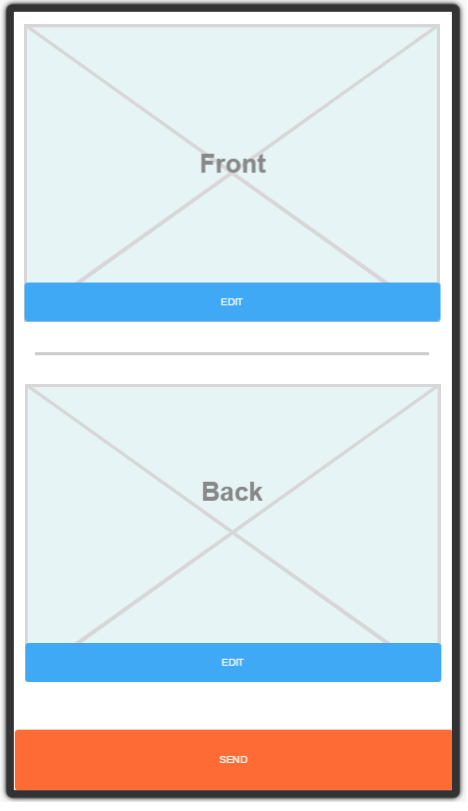
\includegraphics[width=\linewidth]{Prototype_img/p1.png}
		\caption{Start}
		\label{fig:p1}
	\end{minipage}
	\begin{minipage}{0.35\textwidth}
		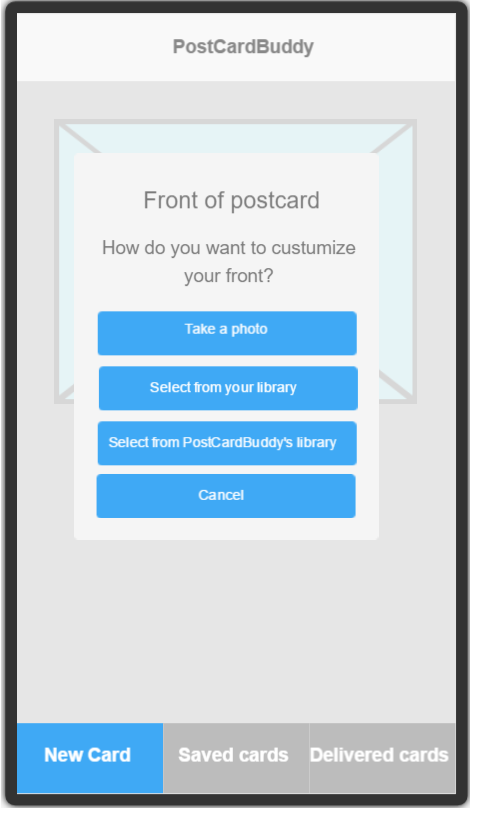
\includegraphics[width=\linewidth]{Prototype_img/p2.png}
		\caption{Chosee image source}
		\label{fig:p2}
	\end{minipage}
	\begin{minipage}{0.35\textwidth}
		
\includegraphics[width=\linewidth]{Prototype_img/p3.png}
		\caption{Image editor}
		\label{fig:p3}
	\end{minipage}
	\begin{minipage}{0.35\textwidth}
		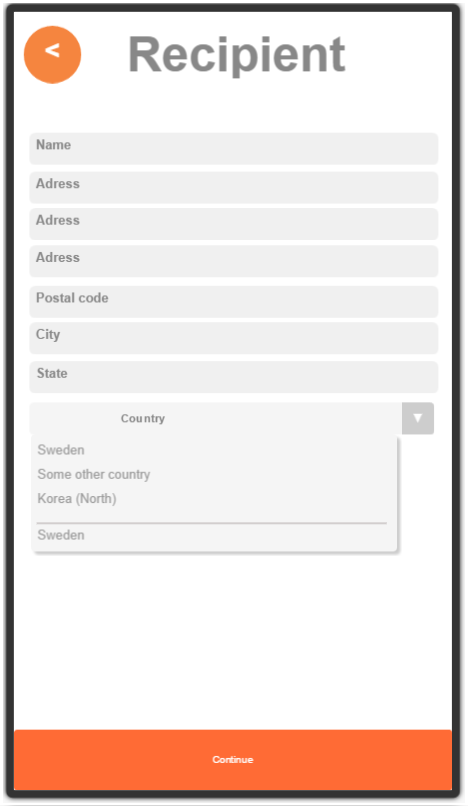
\includegraphics[width=\linewidth]{Prototype_img/p4.png}
		\caption{Recipiant information}
		\label{fig:p4}
	\end{minipage}
\end{figure}

%ref bug?
\item[Req \tsss.6 Start Screen] The application shall start with a screen where its possible to choose front and back image/text figure \ref{fig:p1}.
\item[Req \tsss.7 Get image] The application shall let the user choose the image source from a menu figure \ref{fig:p2}.
\item[Req \tsss.8 Edit image]The application shall give the user a basic image editor to customize the image figure \ref{fig:p3}.
\item[Req \tsss.9 Recipiant address] The application shall have an address input screen with an address-book/contacts (not in image) figure \ref{fig:p4}.
\end{description}

\subsection{Data Requirements}
Short text describing this section.

%TODO: Beskrivning till E/R, data dictionary och virtual window när man skapar vykort.
\begin {description}
\item[Req 1.5.1.1 Data model] The system shall handle the data presented in the data model in figure \ref{fig:datamodel}.
\end{description}

\begin{figure}[h!]
\centering
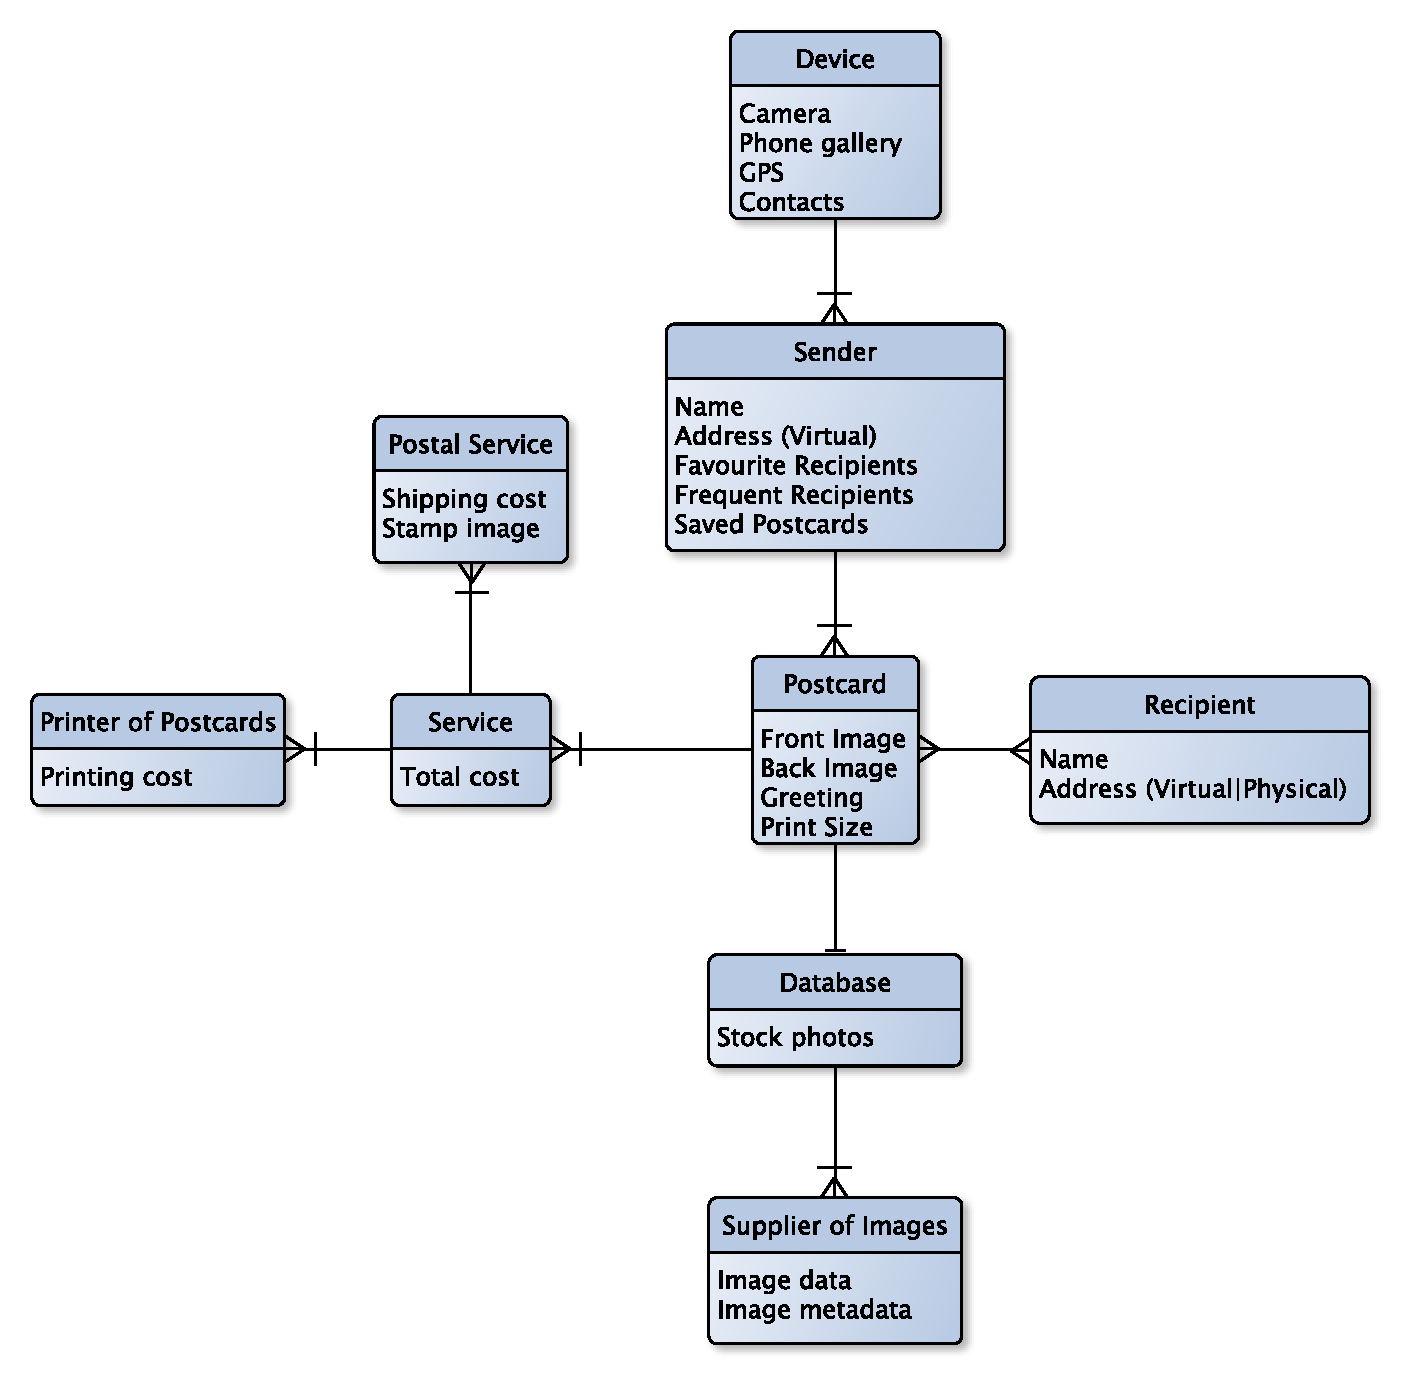
\includegraphics[width=0.7\textwidth]{Data_figures/DataModel.pdf}
\caption{Data model}
\label{fig:datamodel}
\end{figure}

\subsubsection{Data dictionary}

%\begin{description}
%\item[Class:] \textbf{Name} \hfill \\
%Description what it is exactly, what it does and what it interacts with
%
%\item[Examples:] \hfill
%\begin{enumerate}
%\item What is this typically?
%\item Special cases.
%\end{enumerate}
%
%\item[Attributes:] \hfill
%\begin{enumerate}
%\item List attributes and 
%\item What type of data it is
%\end{enumerate}
%\end{description}
%
%\hrulefill

%Do we really support both Android and iOS?
\begin{description}
\item[Class:] \textbf{Device} \hfill \\
The device is the actual physical mobile device on which the application is running.

\item[Examples:] \hfill
\begin{enumerate}
\item An android device running the application.
\item An iOS device running the application
\end{enumerate}

\item[Attributes:] \hfill
\begin{enumerate}
\item \textbf{Camera:} Image \hfill \\A compressed image fetched from the devices physical camera.
\item \textbf{GPS:} String[Latitude,longitude] \hfill \\The information about current coordinates from the GPS in the device. The string is given on the format shown and the latitude and longitudes are signed floats with seven decimal places.
\end{enumerate}
\end{description}

\hrulefill

%Maybe we need to divide virtual and physical in separate attributes. Maybe we need data about what platform to share to?
\begin{description}
\item[Class:] \textbf{Sender} \hfill \\
This class represents the person sending the post card. It can be the same person as the one using the device but it doesn't have to.

\item[Examples:] \hfill
\begin{enumerate}
\item The device owner.
\item A person using the application to send a post card.
\end{enumerate}

\item[Attributes:] \hfill
\begin{enumerate}
\item \textbf{Name:} String \hfill \\The name of the sender. 
\item \textbf{address} (Virtual|Physical): String \hfill \\This attribute is always a string. If it's a virtual address it's a user name, otherwise it's a physical street address. 
\end{enumerate}
\end{description}

\hrulefill

\begin{description}
\item[Class:] \textbf{Receiver} \hfill \\
This class represents the person receiving the post card. This class is identical to \textit{Sender} in terms of attribute structure. The sender and receiver could be the same person.

\item[Examples:] \hfill
\begin{enumerate}
\item The person receiving the post card.
\item The same person as the one sending a post card.
\end{enumerate}
\end{description}

\hrulefill

%Is stamp image required?
\begin{description}
\item[Class:] \textbf{PostCard} \hfill \\
This class represents the the post card sent from the \textit{Sender} to \textit{Receiver}. It encapsulates all the information necessary to send a post card in either virtual or physical form. An instance of this object, owning a \textit{Sender} and a \textit{Receiver} needs to exist to be able to send a Post Card. 

\item[Examples:] \hfill
\begin{enumerate}
\item A post card with two images, a message and a stamp.
\item A post card with no images, no message and a stamp.
\item A virtual post card with images, a message and no stamp.
\end{enumerate}

\item[Attributes:] \hfill
\begin{enumerate}
\item \textbf{Front image:} Image [optional] \hfill \\A compressed image that will be used as the front image of the \textit{PostCard}. 
\item \textbf{Back image:} Image [optional] \hfill \\A compressed image that will be used as the back image of the \textit{PostCard}.
\item \textbf{Message:} String [optional] \hfill \\The message on the \textit{PostCard}.
\item \textbf{Stamp image:} Image \hfill \\The image supplied by \textit{Shipper} to properly send the post card.
\end{enumerate}
\end{description}

\hrulefill

%Maybe we need IDs or names to identify the supplier?
\begin{description}
\item[Class:] \textbf{Suppliers} \hfill \\
This class collects the data from an \textit{Image supplier}, a \textit{Shipper} and a \textit{Printer}. 

\item[Examples:] \hfill
\begin{enumerate}
\item A collection of suppliers relevant to printing and sending a specific \textit{PostCard}.
\item Only a printing and shipping cost.
\end{enumerate}

\item[Attributes:] \hfill
\begin{enumerate}
\item \textbf{Total cost:} Float \hfill \\The combined cost of \textit{Image supplier/Photo cost}, a \textit{Shipper/Shipping cost} and a \textit{Printer/Printing cost}. The value is rounded up to two decimal places.
\end{enumerate}
\end{description}

\hrulefill

\begin{description}
\item[Class:] \textbf{Image supplier:} \hfill \\
This class represents a supplier of images. If a user chooses a stock photo as (for example) a \textit{PostCard/Front image} there is a cost with using the photo that needs to be added to the total cost.

\item[Examples:] \hfill
\begin{enumerate}
\item An image supplier with a photo and a cost.
\item An image supplier with a free photo.
\end{enumerate}

\item[Attributes:] \hfill
\begin{enumerate}
\item \textbf{Photo cost:} Float \hfill \\The cost of a stock photo. The value is rounded up to two decimal places.
\item \textbf{Stock photo:} Image \hfill \\The actual image that will be bought.
\end{enumerate}
\end{description}

\hrulefill

\begin{description}
\item[Class:] \textbf{Shipper:} \hfill \\
This class represents a shipper. The shipper is the company that will transport the post card. 

\item[Examples:] \hfill
\begin{enumerate}
\item A representation of what is required to send a post card with Posten.
\item A representation of what is required to send a post card with DHL.
\end{enumerate}

\item[Attributes:] \hfill
\begin{enumerate}
\item \textbf{Shipping cost:} Float \hfill \\The cost of shipping. The value is rounded up to two decimal places.
\item \textbf{Stock photo:} Image \hfill \\This is the image used on the post card to indicate that shipping was payed for.
\end{enumerate}
\end{description}

\hrulefill

%Unclear who or what the printer actually is.
\begin{description}
\item[Class:] \textbf{Printer:} \hfill \\
This class represents a printer. The printer is responsible for printing the physical post card. 

\item[Examples:] \hfill
\begin{enumerate}
\item A company contracted to print a post card.
\item The company supplying the application.
\end{enumerate}

\item[Attributes:] \hfill
\begin{enumerate}
\item \textbf{Printing cost:} Float \hfill \\The cost of printing. The value is rounded up to two decimal places.
\end{enumerate}
\end{description}


\subsubsection{Virtual windows}
\begin {description}
\item[Req 1.5.1.2 PostCard] The input data to the \textit{PostCard} class described in the Data dictionary shall include the items specified in the virtual window in figure \ref{fig:virtualwindows_postcard}.

\item[Req 1.5.1.3 Sender] The input data to the \textit{Sender} class described in the Data dictionary shall include the items specified in the virtual window in figure \ref{fig:virtualwindows_sender}.

\item[Req 1.5.1.3 Sender] The input data to the \textit{Receiver} class described in the Data dictionary shall include the items specified in the virtual window in figure \ref{fig:virtualwindows_receiver}.

\end{description}
\hfill
%I'll leave this here for now in case a Latex ninja knows what to do. I want to put them in a row, not column.
\begin{centering}
\begin{figure}[!ht]
\begin{minipage}{0.3\textwidth}
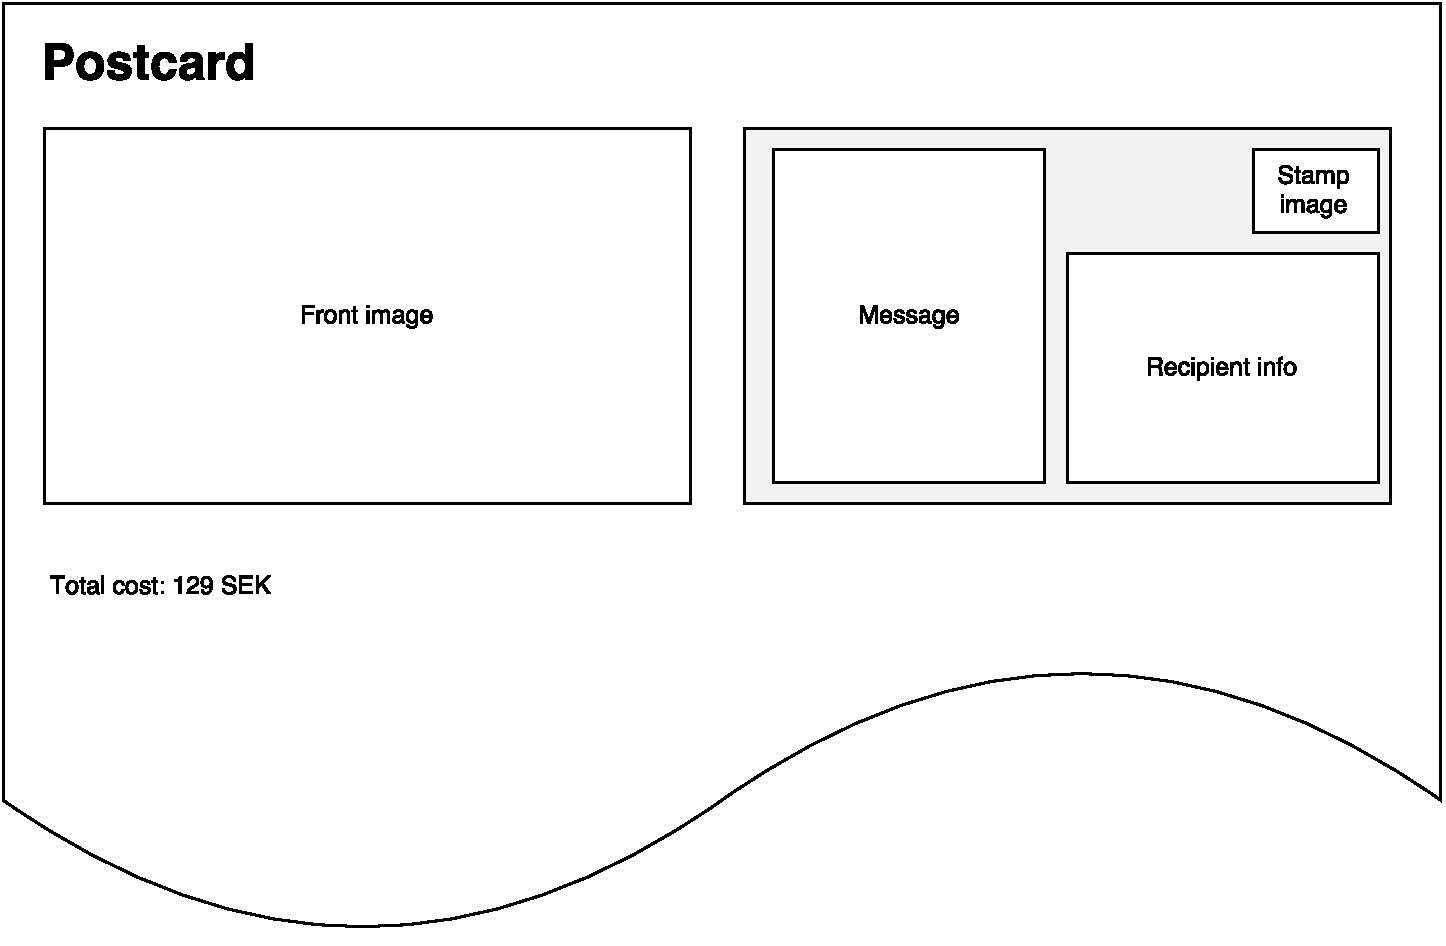
\includegraphics[width=\linewidth]{Data_figures/virtualwindows_postcard.pdf}
\caption{Virtual window PostCard}
\label{fig:virtualwindows_postcard}
\end{minipage}\hfill
~
\begin{minipage}{0.3\textwidth}
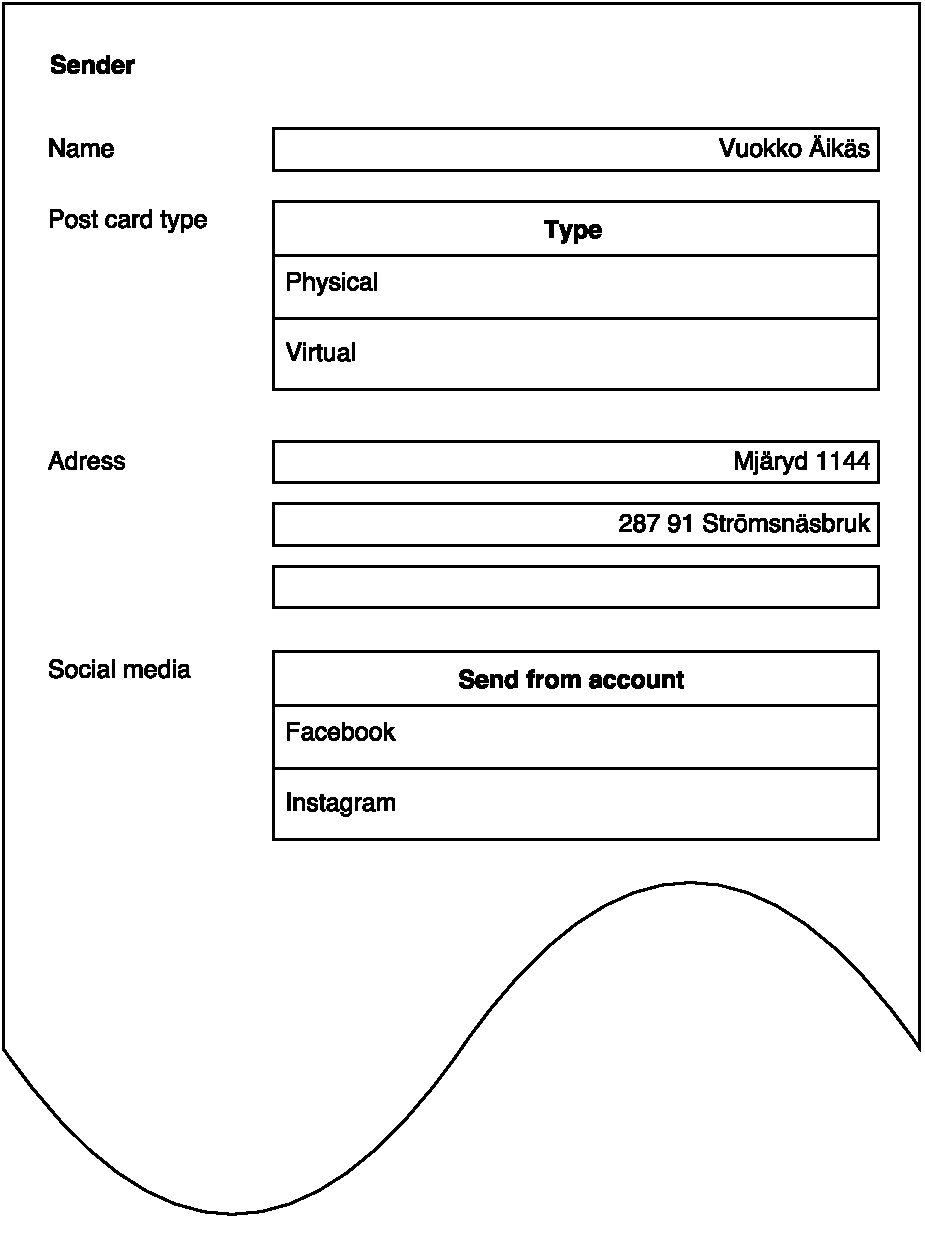
\includegraphics[width=\linewidth]{Data_figures/virtualwindows_sender.pdf}
\caption{Virtual window Sender}
\label{fig:virtualwindows_sender}
\end{minipage}\hfill
~
\begin{minipage}{0.3\textwidth}
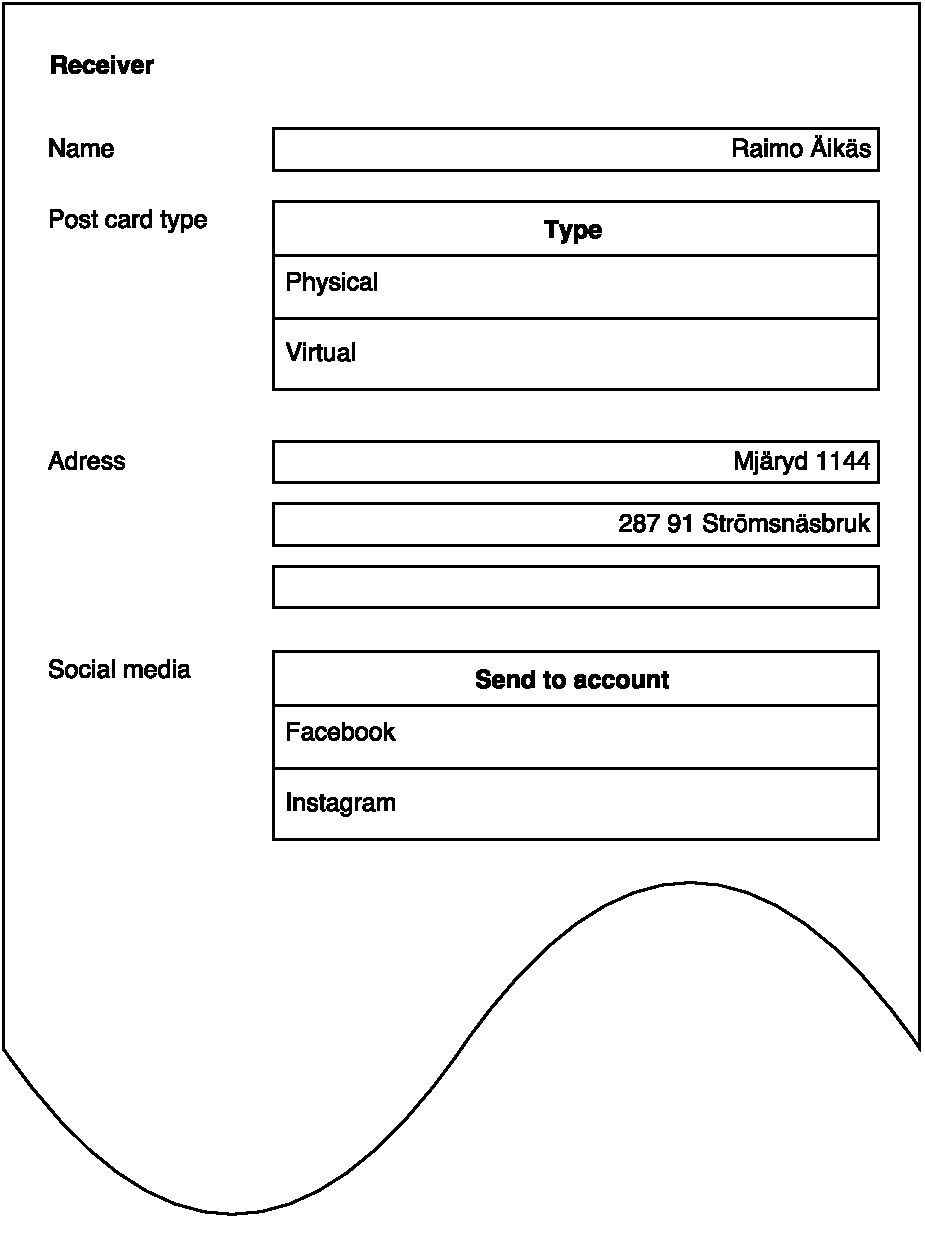
\includegraphics[width=\linewidth]{Data_figures/virtualwindows_receiver.pdf}
\caption{Virtual window Receiver}
\label{fig:virtualwindows_receiver}
\end{minipage}

\end{figure}
\end{centering}

\subsection{Functional Requirements}
\subsubsection{Images} 
\newcounter{images}
\stepcounter{images}
\begin {description}
\item [Req \thesubsubsection {.\theimages} Image from phone gallery]It shall be possible to choose pictures from the phone gallery for the front of the postcard.
\stepcounter{images}
\item [Req \thesubsubsection {.\theimages} Picture from camera] It shall be possible to take a picture through the camera and use as image for the front of the postcard.
\stepcounter{images}
\item [Req \thesubsubsection {.\theimages} Image from standard library] It shall be possible to choose pictures from a standard library.
\stepcounter{images}
\item [Req \thesubsubsection {.\theimages} Image and GPS position] Images from the standard library shall be presented based on the user's GPS position.
\stepcounter{images}
\item [Req \thesubsubsection {.\theimages} Image editing] The system shall have a function for editing of images.
\stepcounter{images}
\item [Req \thesubsubsection {.\theimages} Image saving] It shall be possible to save images.
\end{description}

\subsubsection{Greetings}
\newcounter{greetings}
\stepcounter{greetings}
\begin{description}
\item [Req \thesubsubsection {.\thegreetings} Greetings] It shall be possible to write greetings in the app.
\stepcounter{greetings}
\item [Req \thesubsubsection {.\thegreetings} Pictures of handwritten greetings] It shall be possible to choose a picture of a hand-written greeting.
\stepcounter{greetings}
\item [Req \thesubsubsection {.\thegreetings} Auto-generated greetings] It shall be possible to choose a template greeting.
\stepcounter{greetings}
\item [Req \thesubsubsection {.\thegreetings} GPS based greetings] The system shall be able to generate greetings based on GPS position.
\stepcounter{greetings} 
\item [Req \thesubsubsection {.\thegreetings} Handwritten greetings on screen] It shall be possible to write a handwritten greetings directly on the screen.
\stepcounter{greetings}
%Ovanstående krav onödingt?
\item [Req \thesubsubsection {.\thegreetings} Saving greetings] It shall be possible to save a greeting.
\end{description}

\subsubsection{Recipients}
\newcounter{recipients}
\stepcounter{recipients}
\begin{description}
\item [Req \thesubsubsection {.\therecipients} Enter recipients] It shall be possible to enter recipients manually.
\stepcounter{recipients}
\item [Req \thesubsubsection {.\therecipients} Phone book recipients] It shall be possible to choose recipients through the phone book.
\stepcounter{recipients}
\item [Req \thesubsubsection {.\therecipients} Multiple recipients] The system shall be able to handle multiple recipients for one postcard.
\stepcounter{recipients}
\item [Req \thesubsubsection {.\therecipients} Favourite recipients] It shall be possible to save recipients as favourites.
\stepcounter{recipients}
\item [Req \thesubsubsection {.\therecipients} Frequent recipients] The system shall show frequently used recipients as favourite recipients.
\end{description}

\subsubsection{Postcard}
\newcounter{postcards}
\stepcounter{postcards}
\begin{description}
\item [Req \thesubsubsection {.\thepostcards} Saving postcards] It shall be possible to save postcards.
\stepcounter{postcards}
\item [Req \thesubsubsection {.\thepostcards} Reuse postcards] It shall be possible to reuse saved postcards.
\stepcounter{postcards}

\item [Req \thesubsubsection {.\thepostcards} Preview postcards] It shall be possible to preview postcards before sending it.
\stepcounter{postcards}

\item [Req \thesubsubsection {.\thepostcards} Digital postcard] It shall be possible to send digital postcards.
\stepcounter{postcards}
\item [Req \thesubsubsection {.\thepostcards} Physical postcards] It shall be possible to send physical postcards.
\stepcounter{postcards}

\item [Req \thesubsubsection {.\thepostcards} Payment] It shall be possible to pay for sending physical postcards.
\stepcounter{postcards}

\item [Req \thesubsubsection {.\thepostcards} Postcard size] It shall be possible to choose the size of the physical postcard.
\stepcounter{postcards}
\item [Req \thesubsubsection {.\thepostcards} Quality of physical postcard] It shall be possible to choose the print quality of physical postcards. 
\stepcounter{postcards}
\item [Req \thesubsubsection {.\thepostcards} History] It shall be possible to display the history of sent postcards.

%Ska nedanstående krav vara med?
\item [Req 1.6.3.8 Social media] Feature for sharing postcards on social media.
\end {description}

\subsection{Quality Requirements}



\subsubsection{Quality grid}
Text about quality grid, reference table~\ref{tab:qg}

\begin{table}[h!]
	\centering
	\caption{Quality grid}
	\label{tab:qg}
	\begin{tabular}{|l|l|l|l|l|l|}
		\hline
		\textbf{\begin{tabular}[c]{@{}l@{}}Quality factors -\\ PostCardBuddy\end{tabular}} & \textbf{Critical} & \textbf{Important} & \textbf{As usual} & \textbf{Unimportant} & \textbf{Ignore} \\ \hline
		\textbf{Operation}                                                                 &                   &                    &                   &                      &                 \\ \hline
		Integrity/Security                                                                 &                   &                    & 1                 &                      &                 \\ \hline
		Reliability/availability                                                           &                   & 2                  &                   &                      &                 \\ \hline
		Usability                                                                          & 3                 &                    &                   &                      &                 \\ \hline
		Internet connection demand                                                         & 4                 &                    &                   &                      &                 \\ \hline
		Efficiency                                                                         &                   &                    & x                 &                      &                 \\ \hline
		\textbf{Miscellaneous}                                                             &                   &                    &                   &                      &                 \\ \hline
		Installability                                                                     &                   & 5                  &                   &                      &                 \\ \hline
		Interoperability                                                                   &                   & 6                  &                   &                      &                 \\ \hline
	\end{tabular}
\end{table}

\begin{enumerate}
\item Text about item 1
\item 2
\item 3 etc.
\end{enumerate}

\subsubsection{QUPER}
Text about quper diagram, reference figure~\ref{fig:quper}.


\begin{figure}[h!]
\centering
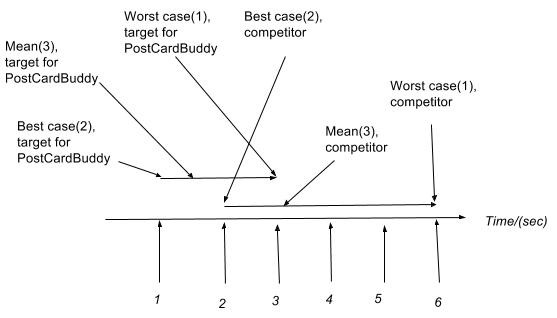
\includegraphics[width=0.7\textwidth]{QUPER_v1.jpg}
\caption{Text about the image here.}
\label{fig:quper}
\end{figure}


\subsubsection{Performance}
\begin{description}
	\item[Req \tsss.1 Memory usage] The application shall adjust its memory usage depending on the device.
	\item[Req \tsss.2 Speed] The user interface shall respond within 200ms after a finished user interaction if there should be an response. This is only applied on devices faster than Nexus 5 / iPhone 5 running original firmware without any other user installed applications on the phone.
	\item[Req \tsss.3 Picture quality] The camera shall be able to take a picture in the highest hardware supported resolution. 
	\item[Req \tsss.4 Autofocus] The camera shall have a autofocus that is comparable to the Android / iOS stock camera. 
\end{description}
\subsubsection{Availability}
\subsubsection{Security}
\begin{description}
	\item[Req \tsss.1 Store cards] The photos shall be stored encrypted
\end{description}
\subsubsection{Maintainability/Portability}
\begin{description}
	\item[Req \tsss.1 Language] The application shall be developed in non native language e.g. Java for Android. 
	\item[Req \tsss.2 Device support] The application shall work on devices with newer operating systems than Android 4.1 / iOS 7.0.1
\end{description}
\subsubsection{Usability}
\begin{description}
	\item [Req \tsss.1 User friendly] 9 out of 10 users shall be able to use the system after a five minute instruction.
\end{description}





%--------------------------------------------------------------------%
%--------------- Specification Techniques ---------------------------%
%--------------------------------------------------------------------%
% Several different specification techniques (e.g. context diagrams, features, virtual windows, task descriptions).

% 3A) apply more than one suitable specification technique (e.g. task descriptions and screen prototypes)
% 4B) use at least four different specification techniques adequately tailored to the context.
% 3B) define a system’s boundaries and its interaction with external entities.
% 5A) combine specification techniques in an explicitly motivated trade off between qualities and costs, where a high degree of specification completeness is achieved for a carefully selected subset of requirements.
% 5C) go beyond initial stakeholders and given frames, while challenging the domain boundaries and eliciting creative ideas and deep domain knowledge in real-world contexts.


%--------------------------------------------------------------------%
%------------------ Release Plan ------------------------------------%
%--------------------------------------------------------------------%
% A release plan defining which requirements that are implemented in each of three releases, namely R3 (final release for this course project), and the imagined future releases R4 and R5. The release plan shall include information used to derive the plan such as priorities and cost.
% The requirements planned for R3 (in the release plan) should be implemented as mock-up designs (e.g. screens and prototypes, analog drawings, clickable presentations, executable gui mockups) and thus included in the final (R3) release.

% 4H) create a release plan for a subset of prioritized features, while taking into account precedence constraints.
% 5F) combine priorities from several stakeholders and use priorities and scheduling constraints to iteratively create a relevant release plan.
\section{Release Plan}




\end{document}

